\chapter{Namespaces}
\section{Why we need Namespaces}
\subsection{Namespaces}


\section{Control Questions A}
\begin{enumerate}
\item Name two* reasons why namespaces are important.\\
So that the processor knows to which Namespace a tag corresponds. Damit wir XML-Dokumente validieren (an ein Schema binden) können.
\item Explain the difference between URLs, URNs and URIs.\\
\begin{center}
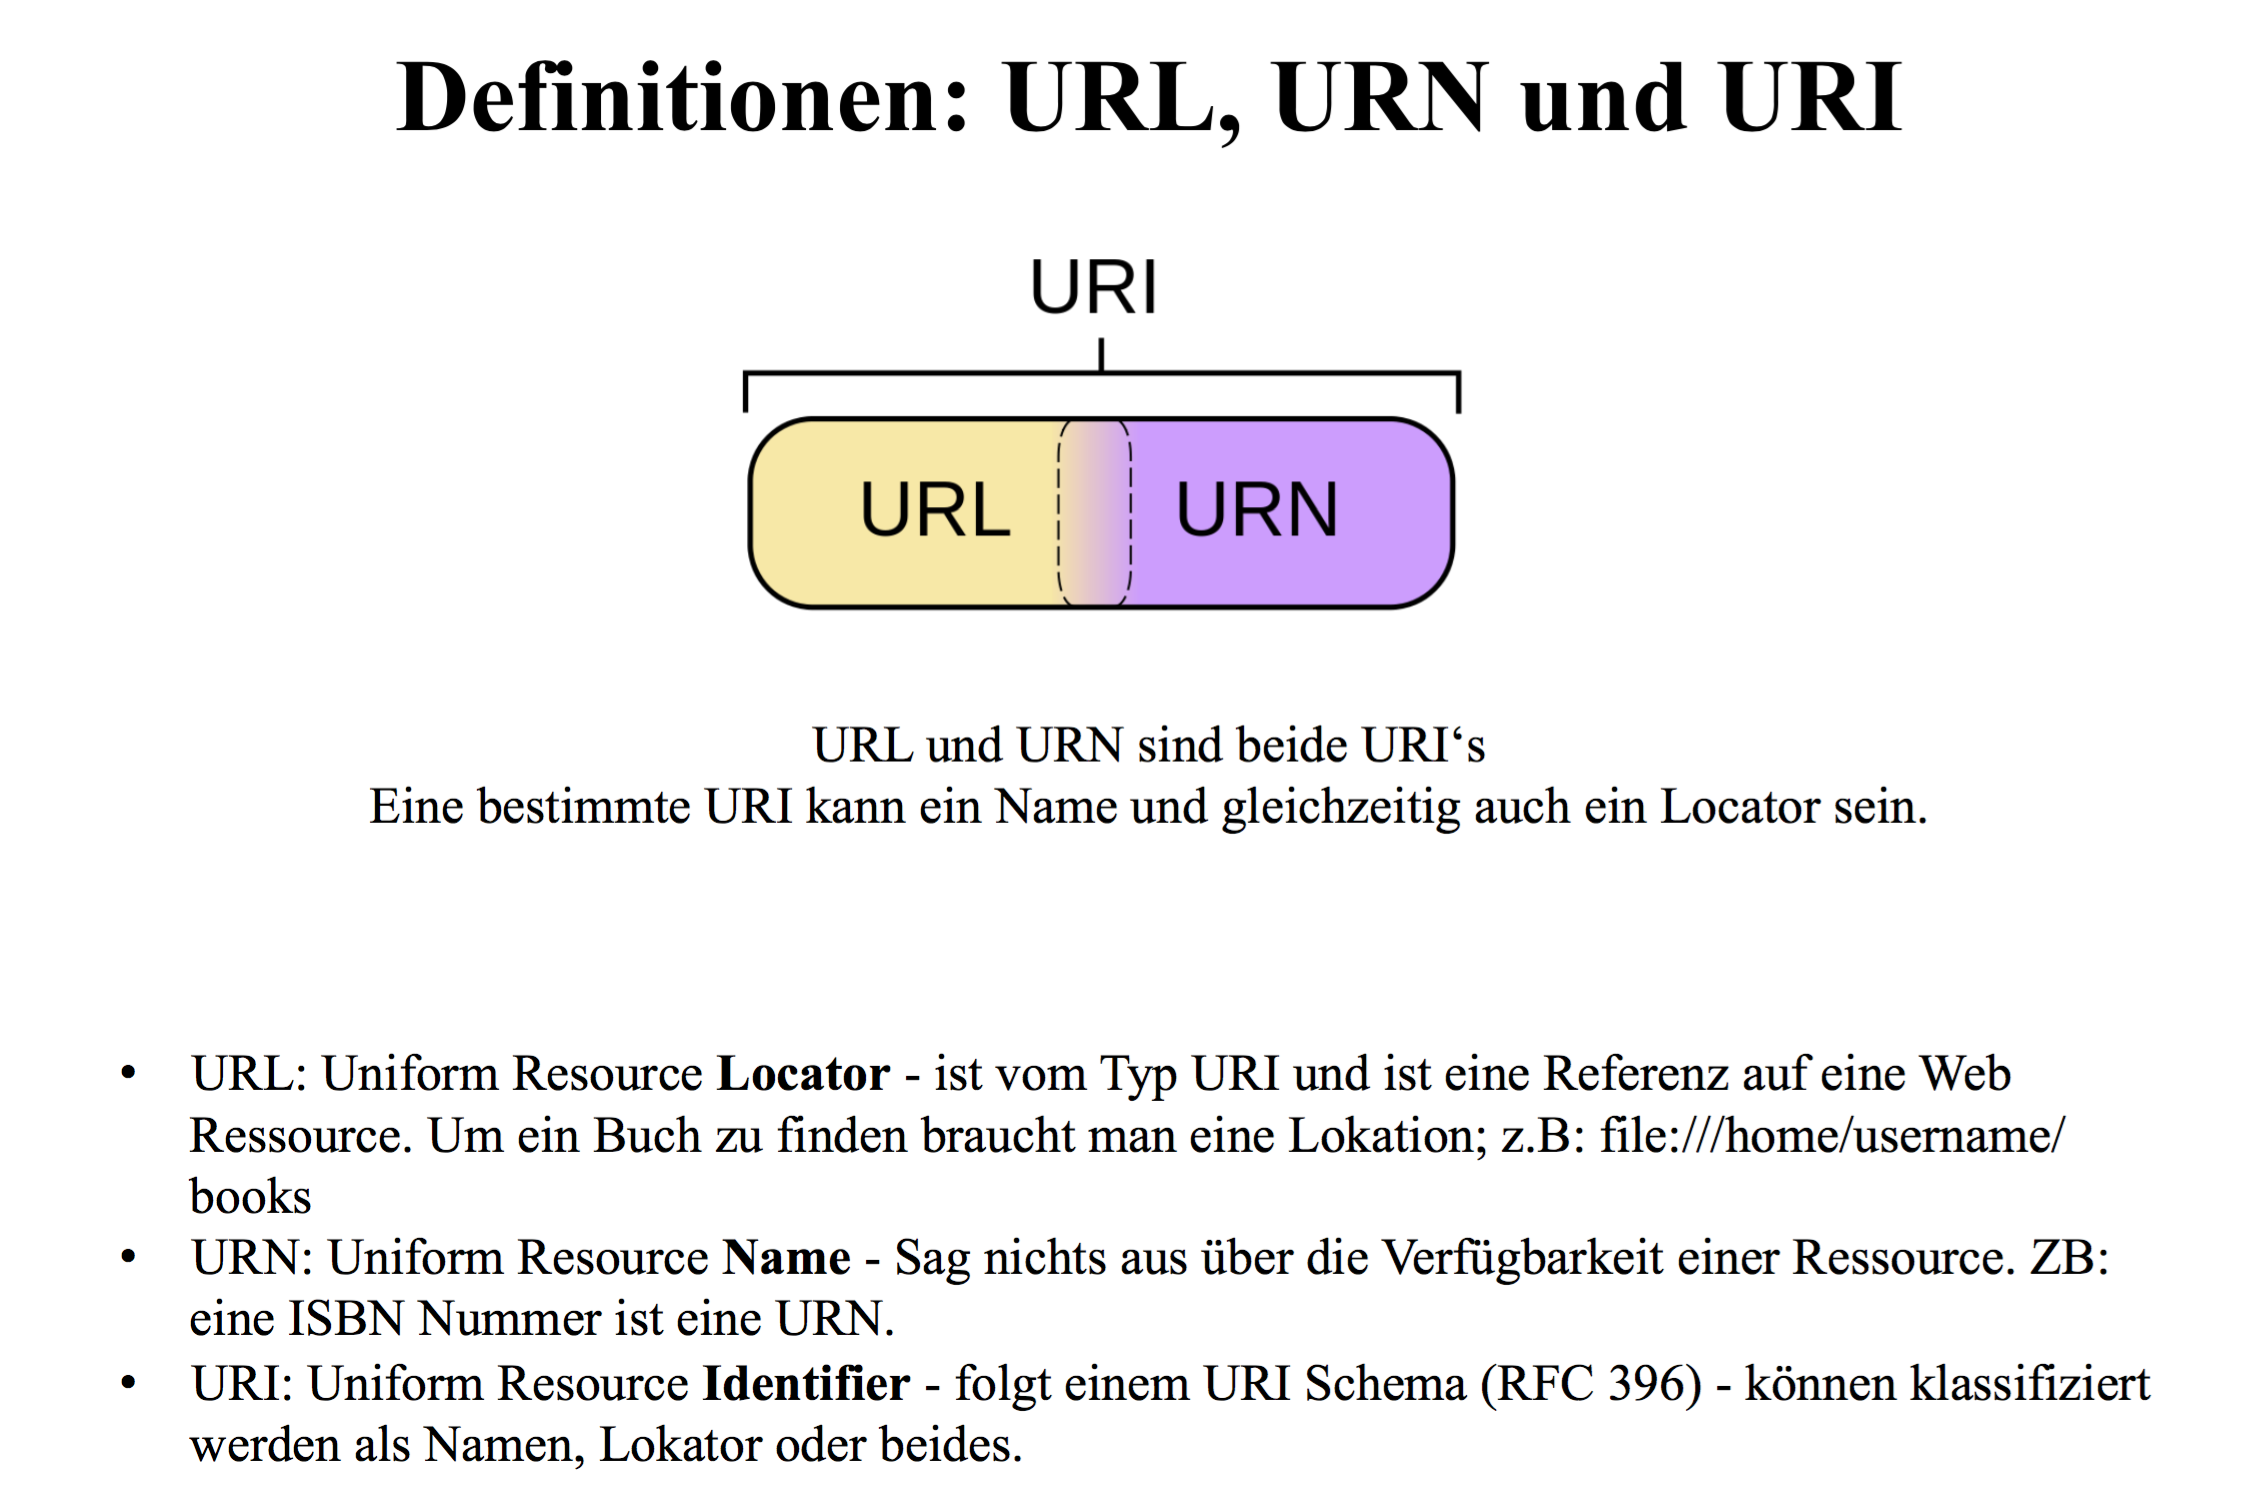
\includegraphics[width=0.7\textwidth]{fig/URI.png}
\end{center}
\item Explain the difference between a default and a prefix namespace.\\
Default Namespace inkludiert alle untergeordneten Tags in diesen Namespace, ein Prefix Namespace muss bei jedem Tag den Namespace angeben.
\item In which regard are attributes special with respect to namespaces ?\\
Attribute nehmen nicht automatisch den Namespace des Default Namespaces an, sondern müssen mit Präfix deklariert werden.
\item What is the XML namespace and why is it special ?\\
Der XML Namespace kann immer verwendet werden (ist automatisch referenziert).
\item Typical exam question on namespaces:
\begin{itemize}
\item Debug an XML document with incorrectly used namespaces
\end{itemize}
\end{enumerate}
